%% bare_jrnl.tex
%% V1.4b
%% 2015/08/26
%% by Michael Shell
%% see http://www.michaelshell.org/
%% for current contact information.
%%
%% This is a skeleton file demonstrating the use of IEEEtran.cls
%% (requires IEEEtran.cls version 1.8b or later) with an IEEE
%% journal paper.
%%
%% Support sites:
%% http://www.michaelshell.org/tex/ieeetran/
%% http://www.ctan.org/pkg/ieeetran
%% and
%% http://www.ieee.org/

%%*************************************************************************
%% Legal Notice:
%% This code is offered as-is without any warranty either expressed or
%% implied; without even the implied warranty of MERCHANTABILITY or
%% FITNESS FOR A PARTICULAR PURPOSE! 
%% User assumes all risk.
%% In no event shall the IEEE or any contributor to this code be liable for
%% any damages or losses, including, but not limited to, incidental,
%% consequential, or any other damages, resulting from the use or misuse
%% of any information contained here.
%%
%% All comments are the opinions of their respective authors and are not
%% necessarily endorsed by the IEEE.
%%
%% This work is distributed under the LaTeX Project Public License (LPPL)
%% ( http://www.latex-project.org/ ) version 1.3, and may be freely used,
%% distributed and modified. A copy of the LPPL, version 1.3, is included
%% in the base LaTeX documentation of all distributions of LaTeX released
%% 2003/12/01 or later.
%% Retain all contribution notices and credits.
%% ** Modified files should be clearly indicated as such, including  **
%% ** renaming them and changing author support contact information. **
%%*************************************************************************


% *** Authors should verify (and, if needed, correct) their LaTeX system  ***
% *** with the testflow diagnostic prior to trusting their LaTeX platform ***
% *** with production work. The IEEE's font choices and paper sizes can   ***
% *** trigger bugs that do not appear when using other class files.       ***                          ***
% The testflow support page is at:
% http://www.michaelshell.org/tex/testflow/



%\documentclass[journal]{IEEEtran}
\documentclass[letterpaper, 10 pt, journal, twoside]{IEEEtran}
%
% If IEEEtran.cls has not been installed into the LaTeX system files,
% manually specify the path to it like:
% \documentclass[journal]{../sty/IEEEtran}





% Some very useful LaTeX packages include:
% (uncomment the ones you want to load)


% *** MISC UTILITY PACKAGES ***
%
%\usepackage{ifpdf}
% Heiko Oberdiek's ifpdf.sty is very useful if you need conditional
% compilation based on whether the output is pdf or dvi.
% usage:
% \ifpdf
%   % pdf code
% \else
%   % dvi code
% \fi
% The latest version of ifpdf.sty can be obtained from:
% http://www.ctan.org/pkg/ifpdf
% Also, note that IEEEtran.cls V1.7 and later provides a builtin
% \ifCLASSINFOpdf conditional that works the same way.
% When switching from latex to pdflatex and vice-versa, the compiler may
% have to be run twice to clear warning/error messages.






% *** CITATION PACKAGES ***
%
%\usepackage{cite}
% cite.sty was written by Donald Arseneau
% V1.6 and later of IEEEtran pre-defines the format of the cite.sty package
% \cite{} output to follow that of the IEEE. Loading the cite package will
% result in citation numbers being automatically sorted and properly
% "compressed/ranged". e.g., [1], [9], [2], [7], [5], [6] without using
% cite.sty will become [1], [2], [5]--[7], [9] using cite.sty. cite.sty's
% \cite will automatically add leading space, if needed. Use cite.sty's
% noadjust option (cite.sty V3.8 and later) if you want to turn this off
% such as if a citation ever needs to be enclosed in parenthesis.
% cite.sty is already installed on most LaTeX systems. Be sure and use
% version 5.0 (2009-03-20) and later if using hyperref.sty.
% The latest version can be obtained at:
% http://www.ctan.org/pkg/cite
% The documentation is contained in the cite.sty file itself.






% *** GRAPHICS RELATED PACKAGES ***
%
\ifCLASSINFOpdf
% \usepackage[pdftex]{graphicx}
% declare the path(s) where your graphic files are
% \graphicspath{{../pdf/}{../jpeg/}}
% and their extensions so you won't have to specify these with
% every instance of \includegraphics
% \DeclareGraphicsExtensions{.pdf,.jpeg,.png}
\else
% or other class option (dvipsone, dvipdf, if not using dvips). graphicx
% will default to the driver specified in the system graphics.cfg if no
% driver is specified.
% \usepackage[dvips]{graphicx}
% declare the path(s) where your graphic files are
% \graphicspath{{../eps/}}
% and their extensions so you won't have to specify these with
% every instance of \includegraphics
% \DeclareGraphicsExtensions{.eps}
\fi
% graphicx was written by David Carlisle and Sebastian Rahtz. It is
% required if you want graphics, photos, etc. graphicx.sty is already
% installed on most LaTeX systems. The latest version and documentation
% can be obtained at: 
% http://www.ctan.org/pkg/graphicx
% Another good source of documentation is "Using Imported Graphics in
% LaTeX2e" by Keith Reckdahl which can be found at:
% http://www.ctan.org/pkg/epslatex
%
% latex, and pdflatex in dvi mode, support graphics in encapsulated
% postscript (.eps) format. pdflatex in pdf mode supports graphics
% in .pdf, .jpeg, .png and .mps (metapost) formats. Users should ensure
% that all non-photo figures use a vector format (.eps, .pdf, .mps) and
% not a bitmapped formats (.jpeg, .png). The IEEE frowns on bitmapped formats
% which can result in "jaggedy"/blurry rendering of lines and letters as
% well as large increases in file sizes.
%
% You can find documentation about the pdfTeX application at:
% http://www.tug.org/applications/pdftex





% *** MATH PACKAGES ***
%
%\usepackage{amsmath}
% A popular package from the American Mathematical Society that provides
% many useful and powerful commands for dealing with mathematics.
%
% Note that the amsmath package sets \interdisplaylinepenalty to 10000
% thus preventing page breaks from occurring within multiline equations. Use:
%\interdisplaylinepenalty=2500
% after loading amsmath to restore such page breaks as IEEEtran.cls normally
% does. amsmath.sty is already installed on most LaTeX systems. The latest
% version and documentation can be obtained at:
% http://www.ctan.org/pkg/amsmath





% *** SPECIALIZED LIST PACKAGES ***
%
%\usepackage{algorithmic}
% algorithmic.sty was written by Peter Williams and Rogerio Brito.
% This package provides an algorithmic environment fo describing algorithms.
% You can use the algorithmic environment in-text or within a figure
% environment to provide for a floating algorithm. Do NOT use the algorithm
% floating environment provided by algorithm.sty (by the same authors) or
% algorithm2e.sty (by Christophe Fiorio) as the IEEE does not use dedicated
% algorithm float types and packages that provide these will not provide
% correct IEEE style captions. The latest version and documentation of
% algorithmic.sty can be obtained at:
% http://www.ctan.org/pkg/algorithms
% Also of interest may be the (relatively newer and more customizable)
% algorithmicx.sty package by Szasz Janos:
% http://www.ctan.org/pkg/algorithmicx




% *** ALIGNMENT PACKAGES ***
%
%\usepackage{array}
% Frank Mittelbach's and David Carlisle's array.sty patches and improves
% the standard LaTeX2e array and tabular environments to provide better
% appearance and additional user controls. As the default LaTeX2e table
% generation code is lacking to the point of almost being broken with
% respect to the quality of the end results, all users are strongly
% advised to use an enhanced (at the very least that provided by array.sty)
% set of table tools. array.sty is already installed on most systems. The
% latest version and documentation can be obtained at:
% http://www.ctan.org/pkg/array


% IEEEtran contains the IEEEeqnarray family of commands that can be used to
% generate multiline equations as well as matrices, tables, etc., of high
% quality.




% *** SUBFIGURE PACKAGES ***
%\ifCLASSOPTIONcompsoc
%  \usepackage[caption=false,font=normalsize,labelfont=sf,textfont=sf]{subfig}
%\else
%  \usepackage[caption=false,font=footnotesize]{subfig}
%\fi
% subfig.sty, written by Steven Douglas Cochran, is the modern replacement
% for subfigure.sty, the latter of which is no longer maintained and is
% incompatible with some LaTeX packages including fixltx2e. However,
% subfig.sty requires and automatically loads Axel Sommerfeldt's caption.sty
% which will override IEEEtran.cls' handling of captions and this will result
% in non-IEEE style figure/table captions. To prevent this problem, be sure
% and invoke subfig.sty's "caption=false" package option (available since
% subfig.sty version 1.3, 2005/06/28) as this is will preserve IEEEtran.cls
% handling of captions.
% Note that the Computer Society format requires a larger sans serif font
% than the serif footnote size font used in traditional IEEE formatting
% and thus the need to invoke different subfig.sty package options depending
% on whether compsoc mode has been enabled.
%
% The latest version and documentation of subfig.sty can be obtained at:
% http://www.ctan.org/pkg/subfig




% *** FLOAT PACKAGES ***
%
%\usepackage{fixltx2e}
% fixltx2e, the successor to the earlier fix2col.sty, was written by
% Frank Mittelbach and David Carlisle. This package corrects a few problems
% in the LaTeX2e kernel, the most notable of which is that in current
% LaTeX2e releases, the ordering of single and double column floats is not
% guaranteed to be preserved. Thus, an unpatched LaTeX2e can allow a
% single column figure to be placed prior to an earlier double column
% figure.
% Be aware that LaTeX2e kernels dated 2015 and later have fixltx2e.sty's
% corrections already built into the system in which case a warning will
% be issued if an attempt is made to load fixltx2e.sty as it is no longer
% needed.
% The latest version and documentation can be found at:
% http://www.ctan.org/pkg/fixltx2e


%\usepackage{stfloats}
% stfloats.sty was written by Sigitas Tolusis. This package gives LaTeX2e
% the ability to do double column floats at the bottom of the page as well
% as the top. (e.g., "\begin{figure*}[!b]" is not normally possible in
% LaTeX2e). It also provides a command:
%\fnbelowfloat
% to enable the placement of footnotes below bottom floats (the standard
% LaTeX2e kernel puts them above bottom floats). This is an invasive package
% which rewrites many portions of the LaTeX2e float routines. It may not work
% with other packages that modify the LaTeX2e float routines. The latest
% version and documentation can be obtained at:
% http://www.ctan.org/pkg/stfloats
% Do not use the stfloats baselinefloat ability as the IEEE does not allow
% \baselineskip to stretch. Authors submitting work to the IEEE should note
% that the IEEE rarely uses double column equations and that authors should try
% to avoid such use. Do not be tempted to use the cuted.sty or midfloat.sty
% packages (also by Sigitas Tolusis) as the IEEE does not format its papers in
% such ways.
% Do not attempt to use stfloats with fixltx2e as they are incompatible.
% Instead, use Morten Hogholm'a dblfloatfix which combines the features
% of both fixltx2e and stfloats:
%
% \usepackage{dblfloatfix}
% The latest version can be found at:
% http://www.ctan.org/pkg/dblfloatfix




%\ifCLASSOPTIONcaptionsoff
%  \usepackage[nomarkers]{endfloat}
% \let\MYoriglatexcaption\caption
% \renewcommand{\caption}[2][\relax]{\MYoriglatexcaption[#2]{#2}}
%\fi
% endfloat.sty was written by James Darrell McCauley, Jeff Goldberg and 
% Axel Sommerfeldt. This package may be useful when used in conjunction with 
% IEEEtran.cls'  captionsoff option. Some IEEE journals/societies require that
% submissions have lists of figures/tables at the end of the paper and that
% figures/tables without any captions are placed on a page by themselves at
% the end of the document. If needed, the draftcls IEEEtran class option or
% \CLASSINPUTbaselinestretch interface can be used to increase the line
% spacing as well. Be sure and use the nomarkers option of endfloat to
% prevent endfloat from "marking" where the figures would have been placed
% in the text. The two hack lines of code above are a slight modification of
% that suggested by in the endfloat docs (section 8.4.1) to ensure that
% the full captions always appear in the list of figures/tables - even if
% the user used the short optional argument of \caption[]{}.
% IEEE papers do not typically make use of \caption[]'s optional argument,
% so this should not be an issue. A similar trick can be used to disable
% captions of packages such as subfig.sty that lack options to turn off
% the subcaptions:
% For subfig.sty:
% \let\MYorigsubfloat\subfloat
% \renewcommand{\subfloat}[2][\relax]{\MYorigsubfloat[]{#2}}
% However, the above trick will not work if both optional arguments of
% the \subfloat command are used. Furthermore, there needs to be a
% description of each subfigure *somewhere* and endfloat does not add
% subfigure captions to its list of figures. Thus, the best approach is to
% avoid the use of subfigure captions (many IEEE journals avoid them anyway)
% and instead reference/explain all the subfigures within the main caption.
% The latest version of endfloat.sty and its documentation can obtained at:
% http://www.ctan.org/pkg/endfloat
%
% The IEEEtran \ifCLASSOPTIONcaptionsoff conditional can also be used
% later in the document, say, to conditionally put the References on a 
% page by themselves.




% *** PDF, URL AND HYPERLINK PACKAGES ***
%
%\usepackage{url}
% url.sty was written by Donald Arseneau. It provides better support for
% handling and breaking URLs. url.sty is already installed on most LaTeX
% systems. The latest version and documentation can be obtained at:
% http://www.ctan.org/pkg/url
% Basically, \url{my_url_here}.

\usepackage{graphics} % for pdf, bitmapped graphics files
\usepackage{epsfig} % for postscript graphics files
%\usepackage{mathptmx} % assumes new font selection scheme installed
%\usepackage{times} % assumes new font selection scheme installed
%\usepackage{amsmath} % assumes amsmath package installed
%\usepackage{amssymb}  % assumes amsmath package installed
\usepackage{booktabs}
\usepackage{graphicx}
\usepackage{siunitx}


% *** Do not adjust lengths that control margins, column widths, etc. ***
% *** Do not use packages that alter fonts (such as pslatex).         ***
% There should be no need to do such things with IEEEtran.cls V1.6 and later.
% (Unless specifically asked to do so by the journal or conference you plan
% to submit to, of course. )


% correct bad hyphenation here
\hyphenation{op-tical net-works semi-conduc-tor}


\begin{document}
	%
	% paper title
	% Titles are generally capitalized except for words such as a, an, and, as,
	% at, but, by, for, in, nor, of, on, or, the, to and up, which are usually
	% not capitalized unless they are the first or last word of the title.
	% Linebreaks \\ can be used within to get better formatting as desired.
	% Do not put math or special symbols in the title.
	\title{Soft Wearable Augmented Walking Suit with Pneumatic Gel Muscles and Stance Phase Detection System to Assist Gait}
	%
	%
	% author names and IEEE memberships
	% note positions of commas and nonbreaking spaces ( ~ ) LaTeX will not break
	% a structure at a ~ so this keeps an author's name from being broken across
	% two lines.
	% use \thanks{} to gain access to the first footnote area
	% a separate \thanks must be used for each paragraph as LaTeX2e's \thanks
	% was not built to handle multiple paragraphs
	%
	
	% \author{Michael~Shell,~\IEEEmembership{Member,~IEEE,}
	%         John~Doe,~\IEEEmembership{Fellow,~OSA,}
	%         and~Jane~Doe,~\IEEEmembership{Life~Fellow,~IEEE}% <-this % stops a space
	% \thanks{M. Shell was with the Department
	% of Electrical and Computer Engineering, Georgia Institute of Technology, Atlanta,
	% GA, 30332 USA e-mail: (see http://www.michaelshell.org/contact.html).}% <-this % stops a space
	% \thanks{J. Doe and J. Doe are with Anonymous University.}% <-this % stops a space
	% \thanks{Manuscript received April 19, 2005; revised August 26, 2015.}}
	\author{Chetan Thakur$^{1}$ Kazunori Ogawa$^{2}$ Toshio Tsuji$^{1}$ Yuichi Kurita$^{1}$%
		\thanks{Manuscript received: February, 25, 2018; Revised May, 29, 2018; Accepted July, 13, 2018.}%Use only for final RAL version
		\thanks{This paper was recommended for publication by Editor Yasuyoshi Yokokohji upon evaluation of the Associate Editor and Reviewers' comments. 
		This research was partially supported by JST PRESTO (JPMJPR16D3) and Grants-in-Aid for Scientific Research KAKENHI (18H03276).
		The author (Chetan Thakur) was supported through the Hiroshima University		TAOYAKA Program for creating a flexible, enduring, peaceful society, funded by the Program for Leading Graduate Schools, Ministry of Education, Culture, Sports, Science and Technology.}  %Use only for final RAL version
		\thanks{$^{1}$Chetan Thakur, Toshio Tsuji and Yuichi Kurita are with Graduate School of Engineering, Hiroshima University, Hiroshima, Japan
			{\tt\footnotesize chetanthakur@hiroshima-u.ac.jp, toshiotsuji@
				hiroshima-u.ac.jp and ykurita@hiroshima-u.ac.jp}}%
		\thanks{$^{2} $Kazunori Ogawa is with Daiya Industries Co. Ltd., Okayama, Japan
	{\tt\footnotesize k.ogawa@daiya-lab.jp}}%
		\thanks{Digital Object Identifier (DOI): see top of this page.}
	}
	% note the % following the last \IEEEmembership and also \thanks - 
	% these prevent an unwanted space from occurring between the last author name
	% and the end of the author line. i.e., if you had this:
	% 
	% \author{....lastname \thanks{...} \thanks{...} }
	%                     ^------------^------------^----Do not want these spaces!
	%
	% a space would be appended to the last name and could cause every name on that
	% line to be shifted left slightly. This is one of those "LaTeX things". For
	% instance, "\textbf{A} \textbf{B}" will typeset as "A B" not "AB". To get
	% "AB" then you have to do: "\textbf{A}\textbf{B}"
	% \thanks is no different in this regard, so shield the last } of each \thanks
	% that ends a line with a % and do not let a space in before the next \thanks.
	% Spaces after \IEEEmembership other than the last one are OK (and needed) as
	% you are supposed to have spaces between the names. For what it is worth,
	% this is a minor point as most people would not even notice if the said evil
	% space somehow managed to creep in.
	
	
	
	% The paper headers
	%\markboth{Journal of \LaTeX\ Class Files,~Vol.~14, No.~8, August~2015}%
	%{Shell \MakeLowercase{\textit{et al.}}: Bare Demo of IEEEtran.cls for IEEE Journals}
	\markboth{IEEE Robotics and Automation Letters. Preprint Version. Accepted July, 2018}
	{Thakur \MakeLowercase{\textit{et al.}}: AWS with PGM and Stance Phase Detection System} 
	
	% The only time the second header will appear is for the odd numbered pages
	% after the title page when using the twoside option.
	% 
	% *** Note that you probably will NOT want to include the author's ***
	% *** name in the headers of peer review papers.                   ***
	% You can use \ifCLASSOPTIONpeerreview for conditional compilation here if
	% you desire.
	
	
	
	
	% If you want to put a publisher's ID mark on the page you can do it like
	% this:
	%\IEEEpubid{0000--0000/00\$00.00~\copyright~2015 IEEE}
	% Remember, if you use this you must call \IEEEpubidadjcol in the second
	% column for its text to clear the IEEEpubid mark.
	
	
	
	% use for special paper notices
	%\IEEEspecialpapernotice{(Invited Paper)}
	
	
	
	
	% make the title area
	\maketitle
	
	% As a general rule, do not put math, special symbols or citations
	% in the abstract or keywords.
%%%%%%%%%%%%%%%%%%%%%%%%%%%%%%%%%%%%%%%%%%%%%%%%%%%%%%%%%%%%%%%%%%%%%%%%%%%%%%%%
\begin{abstract}
	
	The lower limbs of the human body are responsible for human locomotion and maintaining a good quality of life. However, there are many instances of muscle fatigue or injuries caused by stressful work environments, aging, and work that involves walking a long distance. Therefore, there is a need for an assistive suit for walking that can unload muscle efforts during walking and reduce the chances of lower-limb muscle fatigue. In this paper we discuss the development of a lightweight and wearable Augmented Walking Suit (AWS) using Pneumatic Gel Muscle (PGM) and its actuation control using lower limb pose detection mechanism considering the human gait cycle. The objective of this assistive suit is to reduce the required muscle effort of the posterior and anterior muscles during the swing phase of the gait cycle, thereby making it easier to move forward. To evaluate the effects of the AWS, an experiment was conducted to record the surface EMG (sEMG) of eight primary lower limb muscles of seven subjects for two levels of assistive air pressure. The evaluation was done based on the sEMG signal envelope and the statistical difference in the average percentage of maximum voluntary contraction (\%MVC) of the measured muscles. In our result, we found that all muscles showed a statistically significant reduction or no change in muscle activity while wearing the AWS as compared with when the AWS was not worn.
	
\end{abstract}

\begin{IEEEkeywords}
Human Factors and Human-in-the-Loop, Human Performance Augmentation, Soft Material Robotics, Wearable Robots, Pneumatic Actuators
\end{IEEEkeywords}


%%%%%%%%%%%%%%%%%%%%%%%%%%%%%%%%%%%%%%%%%%%%%%%%%%%%%%%%%%%%%%%%%%%%%%%%%%%%%%%%
\section{INTRODUCTION}\label{intro}
\IEEEPARstart{a}{bility} to walk without interruption is one of the critical functions of the human body. It is one of the reasons for enjoying a good quality of life by performing a variety of daily tasks independently. However, there are many instances, such as aging, accidents, and longer and stressful working conditions that result in muscle fatigue and injuries, making it difficult to walk, thereby affecting the quality of life of the individual. Such situations can be avoided or addressed using exoskeletons or wearable assistive devices. The muscle activation pattern of human gait is dynamic, and it changes as the motion or intent is changed, but the basic pattern of the gait cycle remains. While developing the AWS, we considered factors such as the nature of the work area, age, flexibility for use it outdoors, light weight, portability, ease of use, reduced muscle effort during walking, and no impact on the normal gait cycle. With an increasing elderly population and stressful work conditions, devices like this will play a significant role in improving the quality of life. Gar�on et al. \cite{1} mentioned that there is demand for assistive devices for mobility for people such as the elderly, the disabled, and healthcare staff for various tasks involved in daily life. 

Among various lower-limb assistive devices, there is a tradeoff between autonomous actuation, wearability, light weight, and affordability. These are divided in two categories, exoskeletons and exosuits. In case of exoskeletons, HAL \cite{2} makes walking easier for the elderly and supports rehabilitation for post stroke or accidents. Wearable agri robot \cite{3} was designed for supporting farming activities, it supports body posture and reduces the muscle fatigue. A walking assist device was designed for walking with a body weight support system \cite{4} for augmenting walking and assisting the  squatting motion required for pick-and-place tasks in various work environments. The RoboKnee \cite{5} is one degree of freedom (DOF) exoskeleton designed to support human locomotion, such as walking and stair climbing. A plantarflexion assist exoskeleton \cite{6} is designed to reduce the metabolic cost of walking. 

In case of exosuits, a tethered bilateral hip extension and plantarflexion exosuit \cite{7} tested for various assistance magnitude and 22.8\% reduction in metabolic cost of walking was reported. A soft exosuit for hip assistance provides 30\% of the biological torque moment for gait \cite{8} by using a spooled-webbing actuator connected to the back of the thigh. The Myosuit, an untethered biarticular exosuit, reduces the natural knee extension moment during the sit to stand transfer motion by 26\% \cite{9}. Unilateral exosuit support for ankle plantarflexion and dorsiflexion were reported to reduce the metabolic rate of gait by 16\% \cite{10}. A soft inflatable exosuit for knee rehabilitation \cite{11} reduces muscle activity in the rectus femoris by 7\%. A biologically inspired soft exosuit for walking assistance \cite{12} showed an average metabolic reduction of 5.1\% during walking. A passive unpowered exoskeleton reduces metabolic cost of gait by 7\% \cite{13}.


These devices are divided into segments, such as healthcare, disability support, and augmenting locomotion. These devices augment human motion significantly based on the reduction in EMG activities and metabolic rate during walking, but their use in outside environments is limited, especially in agriculture and factory settings. For augmented walking, wearability, light weight, portability, ease of use and reduced muscle fatigue, are essential but together missing in the assistive devices discussed above. To solve this problem, we previously developed a lightweight, low-powered pneumatic gel muscle (PGM) \cite{14} as shown in Fig \ref{fig:pgm}. The PGM can generate force with 60 kPa air pressure, which is not possible with the McKibben pneumatic artificial muscle (PAM) \cite{15}. It is also structured to be stitched to fabric or fixed using Velcro tapes; this makes it easy to design the assistive suit. Fig \ref{fig:pgmelongationratio} shows the relation of the supplied air pressure, generated force, and maximum elongation as a percentage of resting length.

In \cite{16}, we devised the concept of an unplugged powered suit (UPS) for walking assistance using the advantage of the PGM and the gait cycle. The UPS is a passive walking assist suit in which the air pressure required for actuating the PGM is generated by placing a rubber pump at the heel of the shoe. This configuration enables the limb in stance phase to generate the assistive air pressure required for the contralateral limb in the swing phase. The pump in the shoe can generate air pressure up to 50 kPa. The challenges of this configuration as discussed in \cite{14}, the UPS cannot be used for a walking pitch of faster than two steps per second. Another limitation of the UPS is the use of the pump in the shoe. To support multiple muscle groups, more pumps are needed in the shoe, which is not suitable for use in an outside environment because of possible leaks in the pump and the difficulty of walking with pumps in the shoe. In \cite{14} evaluation of the UPS was done based on only four muscles of the lower limb, and only the rectus femoris showed a reduction in muscle activity by 20\% whereas others showed no change. To overcome these challenges of the UPS, we developed the AWS in which an air tank replaces the pumps, and actuation control is designed using force sensitive resistor (FSR) sensors in the shoe. This change solves the problem of supporting variable walking speeds, providing the ability to support multiple muscle groups using additional PGM. 

Here, we discuss the design and control of the AWS, which improves on the UPS by keeping human gait in the loop by using a gait cycle detection system for generating assistive force. In section \ref{methodology} we discuss the PGM and its force characteristics, biomechanics, and human gait detection system, as well as the design and configuration of the AWS. In section \ref{Evaluation}, we discuss the evaluation criteria, experimental method and setups, and results of the lower-limb sEMG evaluation for two levels of assistive force with the comparison of average gait sEMG envelope for all subjects and statistical analysis. Section \ref{discuss} presents the discussion, conclusion, and future works.


\section{Methodology} \label{methodology}

\subsection{Pneumatic Gel Muscle} \label{pgm}
\begin{figure}
	\centering
	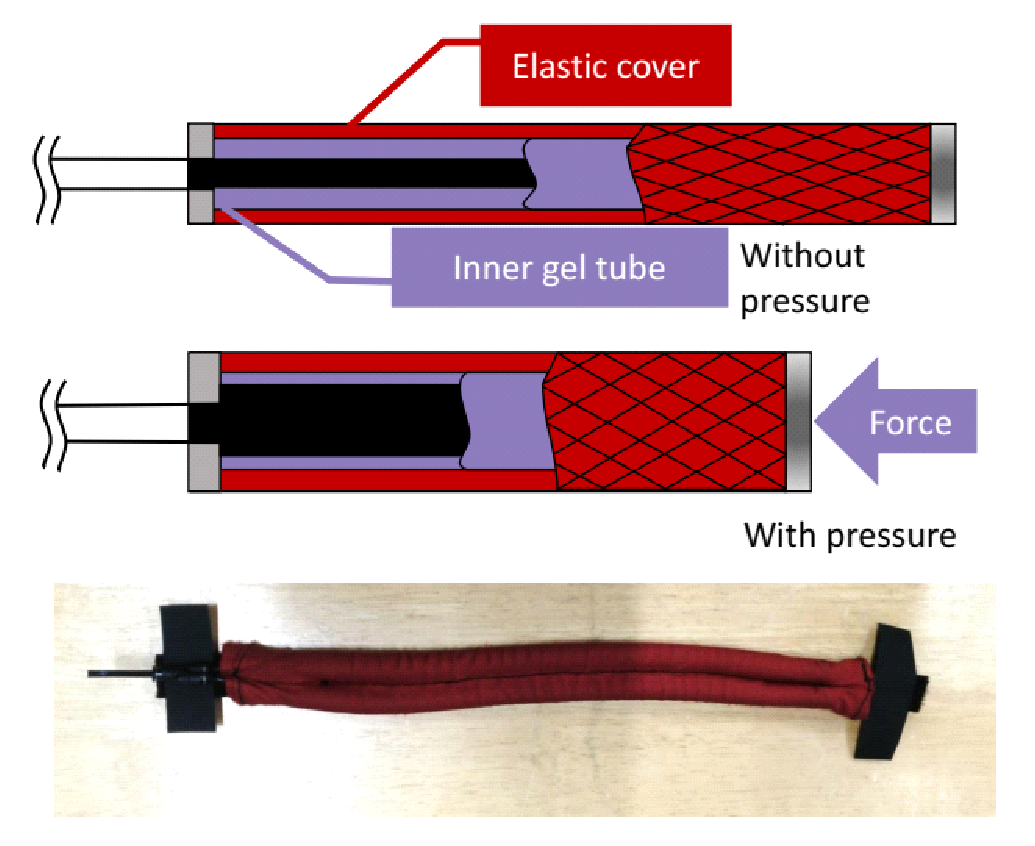
\includegraphics[width=0.9\linewidth]{../photos/pgm}
	\caption{Pneumatic Gel Muscle schematic and prototype. The inner gel tube can be inflated with low air pressure to generate required force. The resting length of the prototype is 30 cm.}
	\label{fig:pgm}
\end{figure}
\begin{figure}
	\centering
	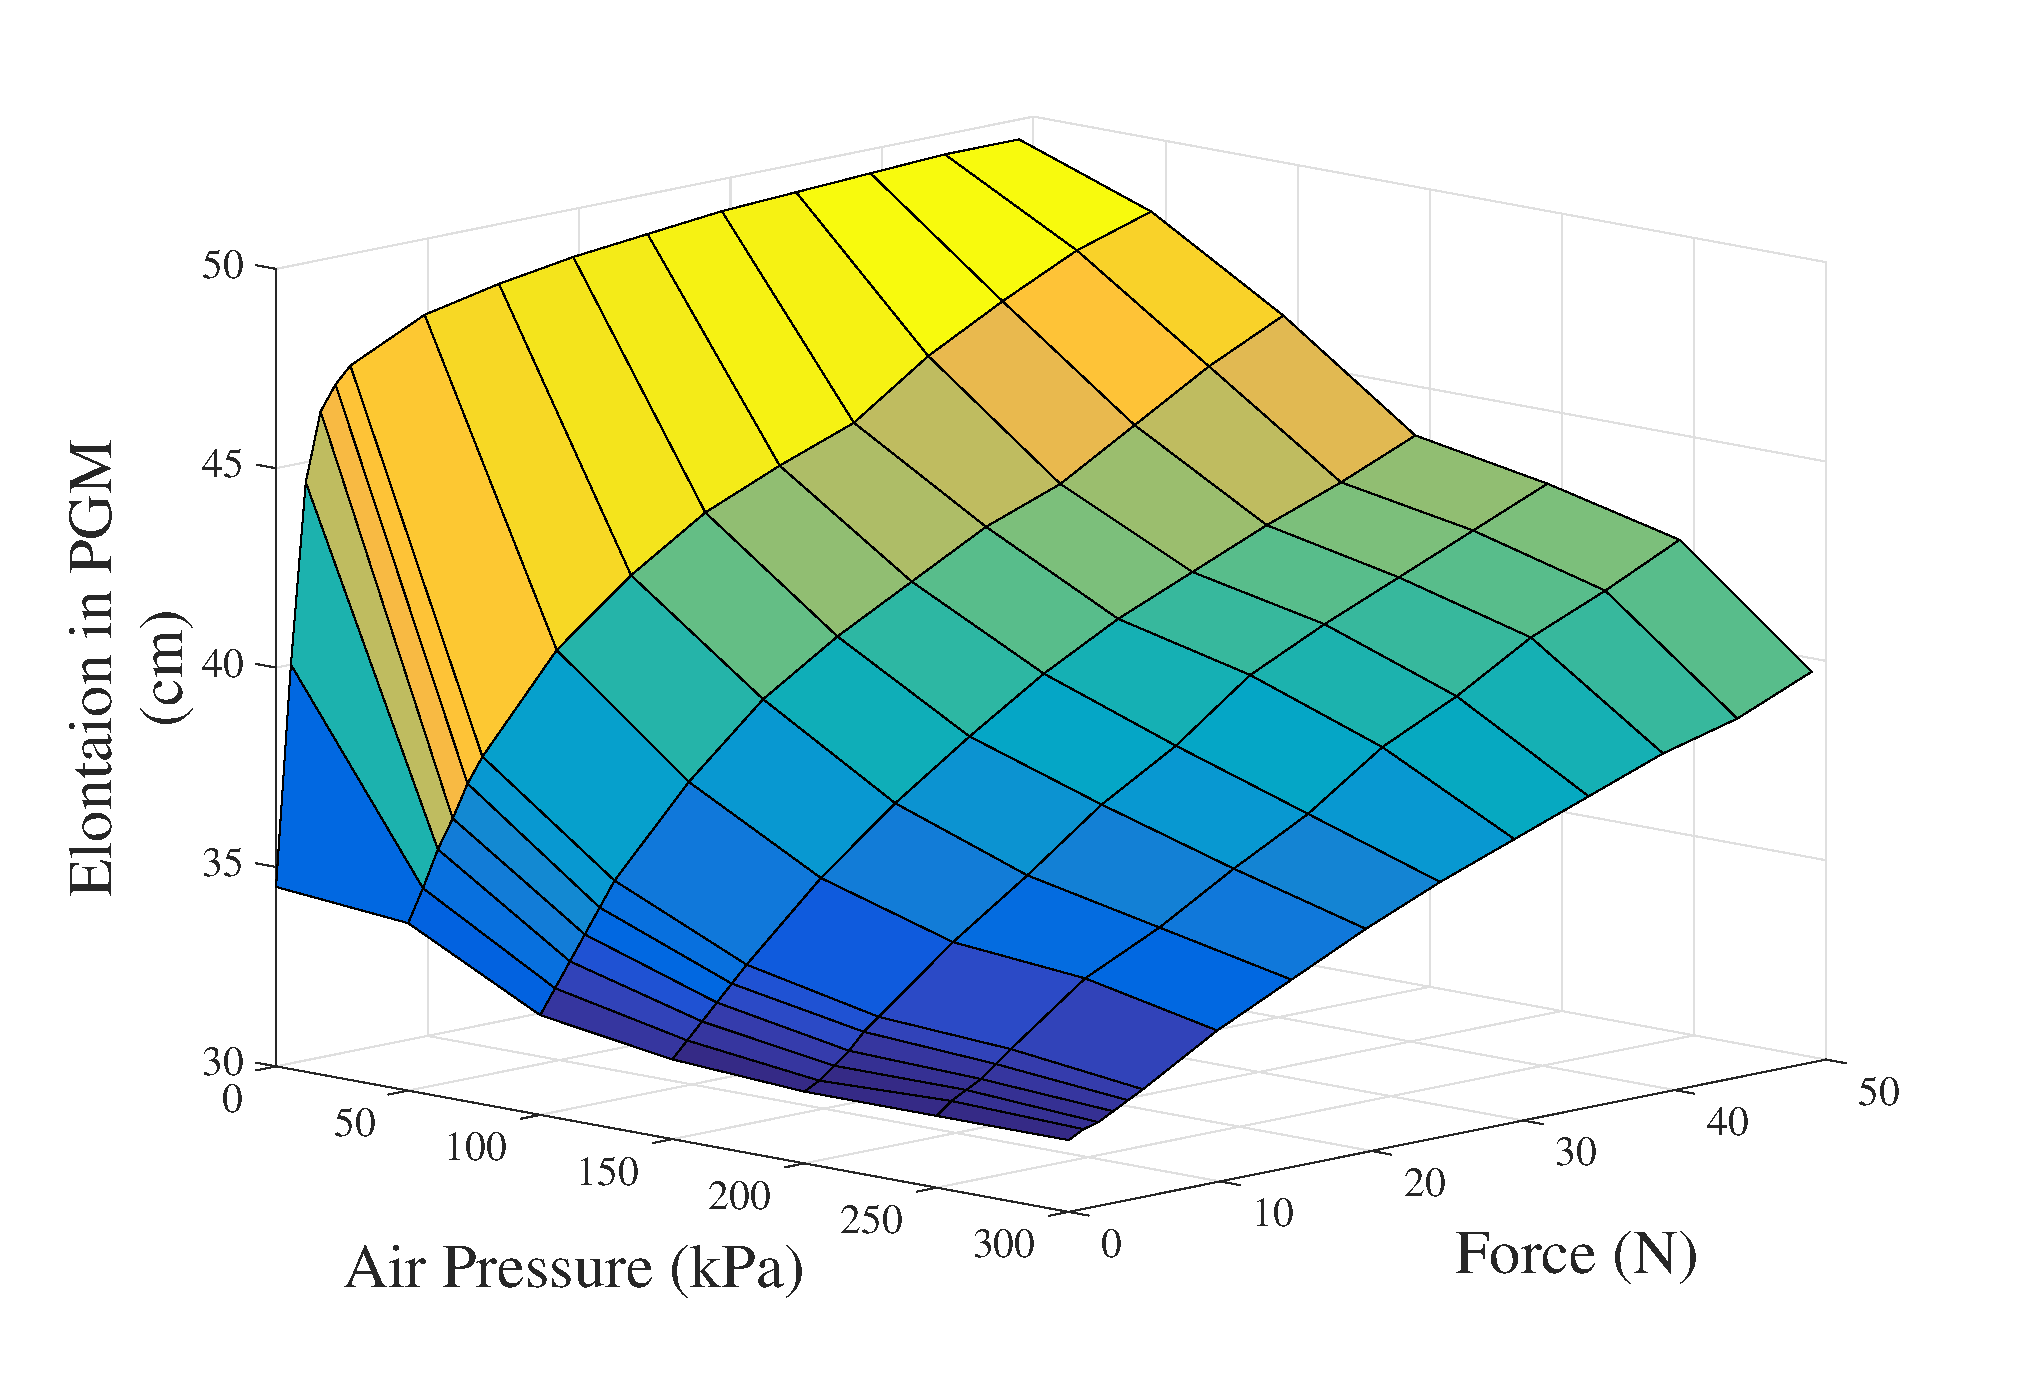
\includegraphics[width=1\linewidth]{../photos/pgmelongation}
	\caption{The graph shows relationship of elongated length of PGM, air pressure and generated force as measured in \cite{14}.}
	\label{fig:pgmelongationratio}
\end{figure}

The PGM is a type of PAM designed to be driven by low air pressure. Fig. \ref{fig:pgm} shows schematics and a prototype of the PGM. It has a resting length of 30 cm, maximum contraction length of 25 cm, and maximum elongation length of 45 cm. Construction of the PGM includes an inner tube made of a unique styrene-based thermoplastic elastomer to improve the flexibility, and an outer protective mesh. The McKibben PAM has rubber or silicone-based rubber tubes covered with protective mesh; these tubes need more air pressure to inflate, whereas the PGM can generate force with air pressure as low as 50 kPa and up to 300 kPa, as reported by \cite{14}. The flexible design and ability to work with low air pressure makes it a more suitable choice for development of wearable assistive suits than the McKibben PAM which has a higher force generating capacity but requires larger air pressure. Fig. \ref{fig:pgmelongationratio} shows the elongation ratio of the PGM as measured by \cite{14}. It shows the force-generating capacity of the PGM and elongation length for various levels of air pressure. In the experiment, one end of the PGM is fixed, and the test load is added to the other end. Whereas, in the AWS both ends of the PGM are fixed and stretched, in this case, the PGM's force-generating characteristics vary. This change is not measured in \cite{14}. Therefore, we conducted an experiment to measure the force generated by the PGM for stretched and un-stretched conditions and different air pressures. The supported range of air pressure is 50 kPa to 300 kPa. Fig. \ref{fig:pgmtest} shows  the experimental setup, where one end is connected to a load cell, and at the other end, the air source is connected through a Panasonic ADP5161 air pressure sensor. The experiment was conducted for two cases unstretched and stretched to 45 cm. Fig. \ref{fig:pgmforceprofile} shows the measured force profile for two conditions in both cases, the PGM shows linear force generation characteristics that are modeled as a linear equations as described in equation \ref{pgmunstreched} and \ref{pgmstreched} with their respective $R^2$ values. These models exhibit similar force generating behavior when used in AWS configuration. These characteristics are useful for controlling assistive force generated by PGM when used in the AWS.

\begin{figure}
	\centering
	\includegraphics[width=1\linewidth]{../photos/forceexpsetup}
	\caption{Experiment setup for studying PGM's force profile.}
	\label{fig:pgmtest}
\end{figure}

\begin{figure}
	\centering
	\includegraphics[width=1\linewidth]{../photos/pgmforceprofile}
	\caption{PGM force profile for unstretched and stretched condition. This represents assistive force applied by PGM when used in AWS based on the input air pressure. In AWS the PGM is stretched along the length of the body segment it is attached. In our experiment we used 60 kPa and 100 kPa assistive air pressure for which approximately 30N and 44N of assistive force was applied by PGM based on the graph above.}
	\label{fig:pgmforceprofile}
\end{figure}


\begin{equation}\label{pgmunstreched}
y=0.1799x - 5.1983; (R^2=0.993)
\end{equation}
\begin{equation}\label{pgmstreched}
y = 0.3883x + 5.8899; (R^2=0.998)
\end{equation}

\subsection{Biomechanics of Gait Cycle } \label{method:gaitcycle}

The design and control of the AWS are based on human walking, i.e., the gait cycle, and depend on how we walk. The gait cycle is divided into three major phases: stance phase, double limb support(DLS) phase and swing phase. The stance phase is responsible for weight acceptance and load transfer to support the swing phase of the contralateral limb. Fig. \ref{fig:standardgait} shows the classification of the gait cycle in the stance and swing phases based on the orientation of the foot. During the transition from one phase to another, there always is a period when both the limbs are on the ground, this is the DLS. In the stance phase, muscle activation of the tibialis anterior (TA), rectus femoris (RF), vastus medialis (VM), vastus lateralis (VL), soleus (SOL), medial gastrocnemius (MG) and lateral gastrocnemius (LG) is observed. These muscles are active from heel strike until toe-off in the stance phase. In the DLS phase, the limb that is transitioning in stance phase supports the forward locomotion of the contralateral limb going in the swing phase. In this phase, both the limbs are on the ground for approximately 10\% of the one gait cycle. SOL, LG, MG, and RF muscles are active and responsible for the limb going into the swing phase. In the swing phase, the limb makes forward movement and RF, VL, VM, and biceps femoris (BF) are the major muscle contributors. 

During the gait cycle, apart from the multiple muscle activation, the position and orientation of the foot also change. The orientation of the foot in the stance phase starts from the heel strike then flat foot, heel-off and ends with toe-off. However, in the swing phase, foot orientation starts from toe-off to heel strike. In DLS, the foot orientations of both limbs contrast with each other, i.e., one limb does heel strike and another does toe-off. This contrast information in DLS is helps to identify the limbs in swing and stance phase. In the AWS we used this information to design an assistive control mechanism to assist the swing phase of the gait cycle, which is discussed in the following subsection.% \ref{method:awscontrol}.


\begin{figure}
	\centering
	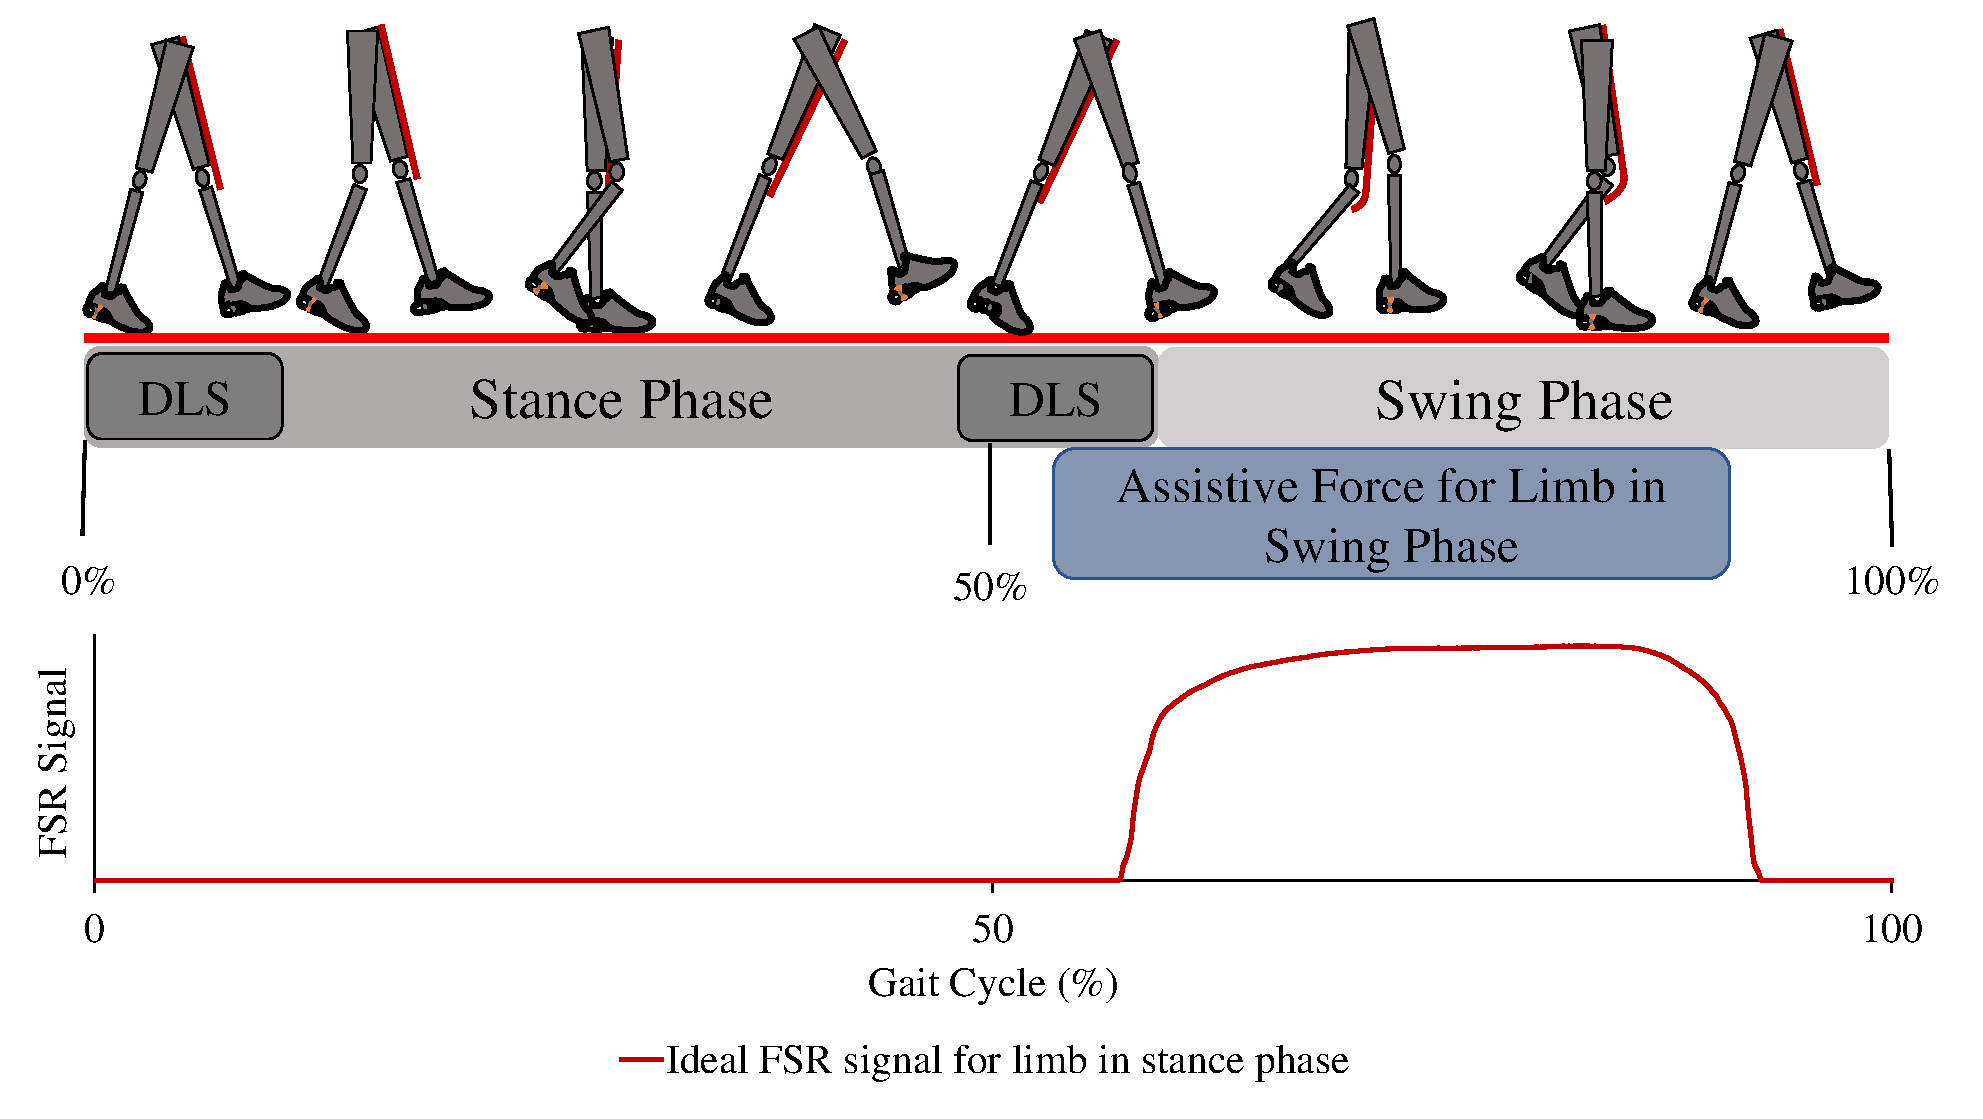
\includegraphics[width=1\linewidth]{../photos/standardGait}
	\caption{The figure shows classification of gait cycle in stance and swing phase along with the double limb support (DLS) which occurs during transition from one phase to another. It also shows the region of assistive gait which starts during double limb support just before initial swing until terminal swing phase. The graph below shows ideal FSR signal from limb in stance phase which assist limb in sing phase.}
	\label{fig:standardgait}
\end{figure}

\subsection{AWS Design and Assistive Control Mechanism} \label{method:awscontrol}

AWS is designed to detect the gait cycle and as shown in Fig. \ref{fig:standardgait} provide assistive force for the limb in the swing phase. To control the assistive force, we placed an FSR-406 sensor in the shoe to detect contrast foot orientation of both limbs in the DLS. The placement of the FSR sensors is shown in Fig. \ref{fig:fsrsole}. This placement helps identify the change in foot orientation while transitioning from the stance to swing phase and vice versa in DLS. By utilizing the knowledge of the gait cycle and the foot orientation from the FSR, we designed the assistive control mechanism for the AWS. Fig. \ref{fig:awssystem} shows the control mechanism of the AWS with the FSR-406 sensor-based stance and swing phase detection mechanism and assistive control. It is a continuous process of proportional (P) control where an Arduino Uno board monitors the FSR sensor data to identify the limbs in the stance and swing phase in the gait cycle. Detection of the limb in the swing phase triggers the assistive control mechanism of the PGM. For actuation control, we used a Kaganei G010E1 3/2 normally closed solenoid valve. The FSR sensor data are continuously monitored for switching ON/OFF solenoid valves. This system is realized using following equation

\begin{figure}
	\centering
	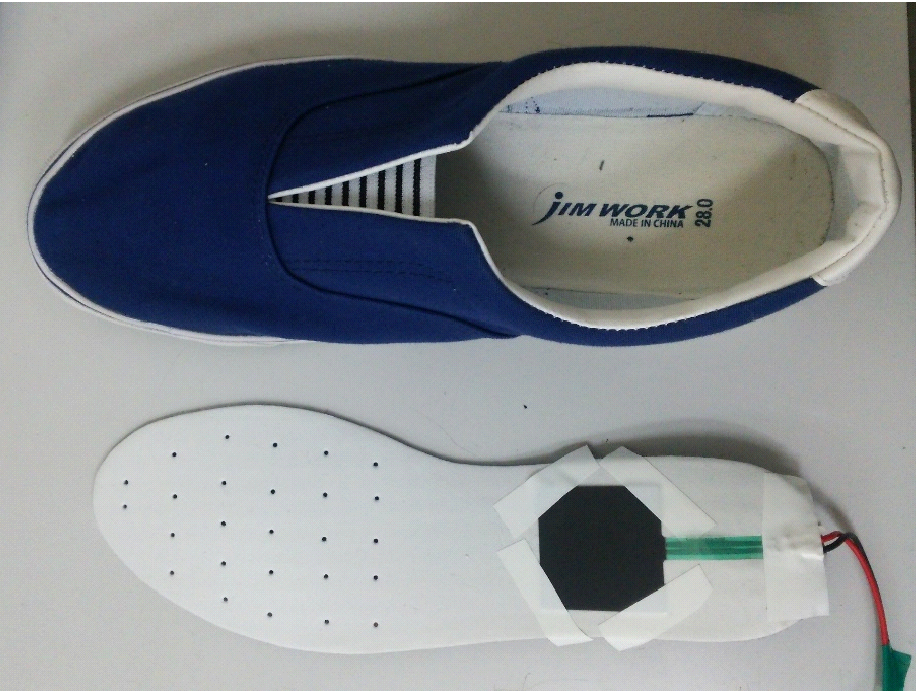
\includegraphics[width=0.3\linewidth]{../photos/fsrsole}
	\caption{The figure shows FSR-406 pressure sensor placement in the shoe. This placement detects the limb in stance and swing phase during DLS}
	\label{fig:fsrsole}
\end{figure}

\begin{figure}
	\centering
	\includegraphics[width=1\linewidth]{../photos/awscontrol}
	\caption{The figure shows AWS assist control mechanism as a continuous process of Proportional (P) control which uses FSR sensor in the shoe to actuate PGM with pneumatic valves connected to portable air tank.}
	\label{fig:awssystem}
\end{figure}

\begin{equation}\label{kevalue}
E = R - Y 
\end{equation}
\begin{equation}\label{uvalue}
U = kpE
\end{equation}

where $E$ is error signal, $R$ is the calibrated threshold value of the FSR sensor, $Y$ is the analog value of the FSR sensor, $U$ is the input to the solenoid valve, and $kp$ is the P-gain. 

The assistive-control mechanism detects the gait cycle by sensing the transition from one phase to another on both limbs in DLS. This way, we avoid unwanted assistive forces during the stationary state where there is no transition. The assistive force generated by the AWS is directly proportional to the supplied air pressure. The supplied air pressure is controlled using the regulator attached to a small air tank used as a source of air pressure.  

\begin{figure}
	\centering
	\includegraphics[width=1\linewidth]{../photos/awsbigfont}
	\caption{The figure shows a subject wearing proposed AWS. The suit consists of backpack with controller, battery and air tank, waist support belt, knee support, two PGMs, pneumatic valves, pressure sensors placed in shoe for controlling assistive force.}
	\label{fig:awsbigfont}
\end{figure}

Fig. \ref{fig:awsbigfont} shows the developed prototype of AWS. AWS consists of waist support and knee support belt for fixing the PGM, PGM along rectus femoris of both limbs, solenoid valves connected to the PGM for actuation control, drawstring backpack which has controller circuit, portable battery and portable air tank. FSR sensors in the shoes are connected to the controller using wires. The weight of the system is 1.2 kg which is lighter than most of the state of the art wearable and portable walking assistive suits. Table \ref{awsweight} shows weights of individual components used in AWS along with total weight of the system.

% Please add the following required packages to your document preamble:
% \usepackage{booktabs}
\begin{table}[]
	\centering
	\caption{Total weight of AWS and its individual parts.}
	\label{awsweight}
	\begin{tabular}{@{}ccc@{}}
		\toprule
		\textbf{Part Name}      & \textbf{Numbers} & \textbf{Weight (kg)} \\ \midrule
		Air Tank with Regulator & 1                & 0.582                  \\
		Solenoid Valve          & 2                & 0.040                   \\
		PGM                     & 2                & 0.110                  \\
		Tubes                   & 1                & 0.022                   \\
		Knee Support Belt       & 2                & 0.052                   \\
		Waist Support Belt      & 1                & 0.108                  \\
		Controller and wires    & 1                & 0.303                  \\ \midrule
		Total                   &                  & 1.217                 \\ \bottomrule
	\end{tabular}
\end{table}

\section{AWS Performance Evaluation through Muscle Activation Pattern of Lower-Limb Muscles} \label{Evaluation}

To test our assumption that the newly developed AWS can assist walking and that change in assistive air pressure reduces muscle activity in lower-limb muscle groups, the experiment was conducted to test the performance evaluation of the AWS with two levels of assistive air pressure. 

Walking involves a combination of muscle activation dynamics of the anterior and posterior lower limb muscles. These changes were recorded using sEMG signals of eight major posterior and anterior muscles that contribute to the gait cycle. We measured TA, SOL, MG, LG, RF, VM, VL, and BF. These muscles are superficially accessible to record sEMG of the lower limb and collectively support the gait cycle. The performance of the AWS is measured based on the statistical difference in the sEMG recorded when the subject was not wearing the AWS and wearing the AWS with two levels of assistive air pressure.


\subsection{Experiment Protocol}
To evaluate the effect of the AWS on the muscle activation pattern of lower-limb muscles for two levels of assistive air pressure, the device was tested on a group of seven healthy young subjects with no gait abnormalities. The subject's age ($\pm$ SD) was 28.8 $\pm$ 5.1, height was 150 $\pm$ \SI{10}{\centi\meter}, and weight was 70.8 $\pm$ \SI{14.5}{\kilogram}. All the subjects participated in the experiment after a brief introduction of the AWS and experiment requirements.

For effective evaluation of the assisted gait, we need to measure a minimum of three full gait cycles \cite{17}.
In our experiment, we recorded sEMG for ten full gait cycles. This was done by asking subjects to walk 15 m straight on a flat surface by maintaining the walking speed during all experiments. The sEMG and FSR sensor data were logged using Personal EMG (P-EMG) device from Oisaka electronic Ltd. For continuous and uninterrupted walking and recording of the data during the experiment, we prepared a backpack containing the P-EMG device, portable battery, and a laptop to operate the P-EMG device. The backpack also contained a controller circuit for the AWS and portable air tank. The laptop was accessed remotely to record the sEMG. Fig. \ref{fig:experimentsetup} shows the experimental setup with the backpack. The total weight of the backpack during experimental evaluation was \SI{6}{\kilogram}.% Before starting the experiment, we recorded MVC for each muscle under observation for all subjects. Exercises such as squat for BF; calf raises for SOL, LG, and MG; thigh contraction for RF, VM, and VL; and ankle dorsiflexion for TA are used to record MVC.%

With the above setup, we conducted three experiments to evaluate the AWS. In the first, sEMG data were recorded for a normal gait, i.e., when subjects were not wearing the AWS. This data gave us the baseline for evaluating the effects of the AWS. In the second and third experiments, sEMG data were recorded for the assisted gait, i.e., subjects wearing the AWS with the backpack containing the experimental setup. For all subjects sEMG of right lower limb was measured for two levels of assistive air pressure during this experiment, i.e. \SI{60}{\kilo\pascal} and \SI{100}{\kilo\pascal} respectively. Three iterations of each experiment were performed to record enough data to conduct a statistical analysis. 




\begin{figure}
	\centering
	\includegraphics[width=1\linewidth]{../photos/awsexperiment}
	\caption{Experiment setup, subject wearing AWS, electrodes and backpack. The backpack contains sEMG recording device, laptop, controller for the AWS, portable battery for controller and sEMG recording device. The total weight of the backpack is \SI{6}{\kilogram}.}
	\label{fig:experimentsetup}
\end{figure}

\subsection{Results}

The recorded sEMG was rectified with integrated EMG (iEMG), a second-order low-pass filter with a cut-off frequency of \SI{100}{\hertz}, and a second-order high-pass filter with a cut-off frequency of \SI{40}{\hertz} using the P-EMG plus tool for the P-EMG device. The recorded sEMG was normalized using MVC to find \%MVC, and ten gait cycles for each subject were averaged to create one gait cycle which is further averaged to generate one gait cycle of all subject. The segmentation of gait cycle was done from stance to stance detection on the left limb based on FSR sensor data in P-EMG tool. This was done because in AWS the stance phase of one limb assists swing phase of the contralateral limb. We measured standard deviation and performed statistical analysis using a two-sample t-test on the average normalized sEMG for all muscles under observation.

Fig. \ref{fig:emgenvelope} shows the normalized average sEMG signal envelope for all subjects with standard deviation of the gait cycle without wearing AWS and wearing AWS with two levels assistive air pressure at \SI{60}{\kilo\pascal} and \SI{100}{\kilo\pascal}. The gait cycle reference for the sEMG signal is swing to swing phase of the right limb. The figure also shows the FSR sensor data for both limbs. The signal peak shows the stance phase on the respective limb and swing on the contralateral limb. AWS detects stance phase on the left and assists swing phase of the right limb (during the experiment we measured sEMG of the right limb). From the graphs, we see that, as we increase the assistive air pressure reduction in the peak value of the normalized averaged sEMG signal not only in the swing phase but also in the stance phase. To evaluate the differences quantitatively, we conducted a two-sample t-test between unassisted gait when AWS was not worn and assisted gaits. Fig. \ref{fig:aggregatedbargraph} shows averaged \%MVC for the three experiments and their significance for individual muscles. 

All the muscles showed significant reduction or no change in the muscle activity evaluated during the experiment. Muscles showed reduction for both levels of assistive air pressure. Table \ref{t-test} shows the result of the two-sample t-test showing the significance of the reduction in the muscle activity based on $p-value$. The Table \ref{percentred} shows percentage reduction in muscle activity. TA, LG, RF, VL and BF shows larger reduction in \%MVC while for SOL, MG and VM shows reduction less than 10\% of \%MVC. From the data in both the tables we observe that assisting swing phase by controlled actuation reduces muscle activity of the measured muscles of the lower limb. 

Therefore, based on the results and analysis we found that the AWS developed in this study can augment human gait as compared to when no AWS is worn. The AWS was able to reduce the muscle efforts significantly in both levels of assistive air pressure by assisting swing phase of the gait cycle. 


\begin{figure*}
	\centering
	\includegraphics[width=0.7\linewidth]{../photos/emgenvelopewithfsr}
	\caption{The figure shows normalized averaged sEMG signal envelope for lower limb muscle groups observed for walking when AWS is not worn and when AWS is worn with two levels of assistive air pressure. It also shows FSR sensor signal showing assistive phase in the gait cycle. The X-axis is the percentage gait cycle (heel strike to heel strike). The Y-axis of the FSR signal is voltage out recorded on the P-EMG device, and for the muscle group, it is average percentage MVC recorded during the experiment.}
	\label{fig:emgenvelope}
\end{figure*}

\begin{figure*}
	\centering
	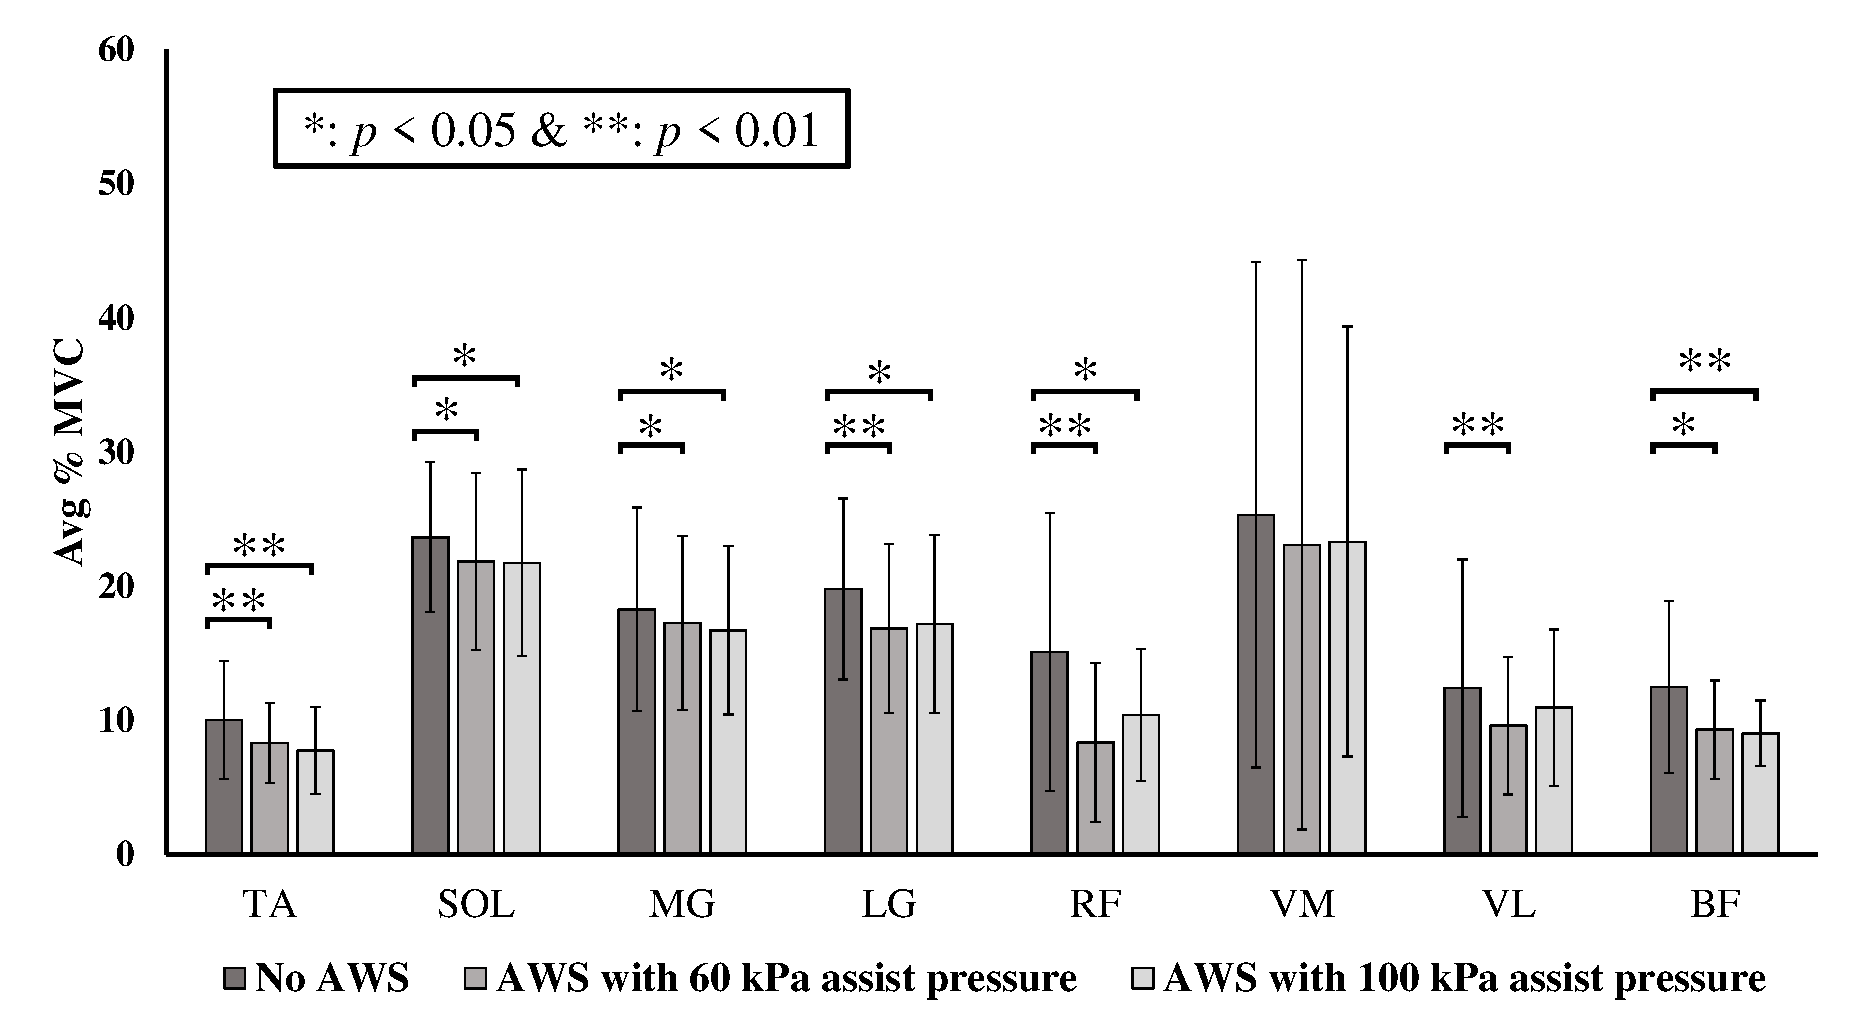
\includegraphics[width=0.8\linewidth]{../photos/aggregatedbargraph}
	\caption{The figure shows the significance of the reduction in \%MVC of the muscle groups for unassisted and assisted with two level of assistive force. The result shows significant reduction or no change in the muscle activation during assisted walking recorded for seven subjects.}
	\label{fig:aggregatedbargraph}
\end{figure*}

% Please add the following required packages to your document preamble:
% \usepackage{booktabs}
\begin{table}[]
	\centering
	\caption{Result of two sample t-test with the respective p-value, t-value and t-critical. P-values are marked with * ($<0.05$) or ** ($<0.01$) as displayed in Fig. \ref{fig:aggregatedbargraph}.}
	\label{t-test}
	\begin{tabular}{@{}cllcc@{}}
		\toprule
		\textbf{Muscles} & \multicolumn{1}{c}{\textbf{Experiment}} & \multicolumn{1}{c}{\textit{\textbf{p-value}}} & \textit{\textbf{t-value}} & \multicolumn{1}{c}{\textit{\textbf{t-critical}}} \\ \midrule
		TA               & AWS 60 Kpa                              & 0.0001 **                                     & 14.51                     & 2.78                                             \\
		& AWS 100 Kpa                             & 0.0002 **                                     & 24.25                     & 3.18                                             \\
		SOL              & AWS 60 Kpa                              & 0.0392 *                                      & 3.02                      & 2.78                                             \\
		& AWS 100 Kpa                             & 0.0329 *                                      & 3.20                      & 2.78                                             \\
		MG               & AWS 60 Kpa                              & 0.0310 *                                      & 3.85                      & 3.18                                             \\
		& AWS 100 Kpa                             & 0.0116 *                                      & 4.41                      & 2.78                                             \\
		LG               & AWS 60 Kpa                              & 0.0095 **                                     & 4.68                      & 2.78                                             \\
		& AWS 100 Kpa                             & 0.0201 *                                      & 4.53                      & 3.18                                             \\
		RF               & AWS 60 Kpa                              & 0.0079 **                                     & 6.35                      & 3.18                                             \\
		& AWS 100 Kpa                             & 0.0420 *                                      & 4.72                      & 4.30                                             \\
		VM               & AWS 60 Kpa                              & 0.0670                                        & 2.50                      & 2.78                                             \\
		& AWS 100 Kpa                             & 0.3300                                        & 1.16                      & 3.18                                             \\
		VL               & AWS 60 Kpa                              & 0.0075 **                                     & 6.46                      & 3.18                                             \\
		& AWS 100 Kpa                             & 0.4003                                        & 1.06                      & 4.30                                             \\
		BF               & AWS 60 Kpa                              & 0.0192 *                                      & 7.11                      & 4.30                                             \\
		& AWS 100 Kpa                             & 0.0020 **                                     & 10.16                     & 3.18                                             \\ \bottomrule
	\end{tabular}
\end{table}

\section{Discussion} \label{discuss}

Our results show that the previously developed PGM can be used for the development of the AWS and make it lightweight, portable, and easy to use. The use of the AWS showed a reduction in the muscle activity in all the major lower-limb muscles. Because of the soft nature of the suit this device does not drastically disturb the normal gait of the wearer. 

The assistive control developed for the AWS detects limbs going in the stance and swing phase during DLS by sensing the FSR sensor data. The simple P control supports 20\%-30\% of the gait cycle during the swing phase.  Because of the nature of the gait cycle and power source for the actuator, it is easy to add additional PGMs to the AWS to increase  range of the assistive force. It is also possible to support the stance and swing phase on a contralateral limb using same solenoid valve, since in the standard gait cycle both limbs functions synchronously.
The device uses waist and knee support to attach the PGM along the rectus femoris muscle. This position sometimes a causes little disturbance during walking. It can be addressed by changing the way PGMs are attached to the limbs in a way such that it does not disturb the degree of freedom at the knee or any other joint when the PGMs are used. 

State-of-the-art wearable walking assist suits are inspired by the biological function of walking, and the assistive actuators aligned with the muscles and joints of the lower limb \cite{8} .. \cite{13}. In such devices, the swing phase of the gait is assisted with an actuators attached close to the ankle or along the soleus muscle and a reduction in the metabolic cost of walking is demonstrated. In our research, AWS is developed to assist the swing phase PGM is attached along the RF muscle from hip to knee, and experimental evaluation shows a progressive reduction in the muscle activity of TA, SOL, MG, and LG. Along with this, RF, VL, and BF also show a reduction in muscle activity. 

Qualitatively, from the oral feedback from subjects, we found that the device is lightweight when not using the 6 kg experimental setup; subjects also reported feeling the assistive force of the PGM during the swing phase of the gait cycle. Some subjects reported sense of assistive force during walking when assistive air pressure changed to 100 kPa as compared to 60 kPa. They also reported that the PGM attachments do not disturb the walking experience but improving the attachment at the knee can result in a more comfortable walking experience.

% Please add the following required packages to your document preamble:
% \usepackage{booktabs}
\begin{table}[]
	\centering
	\caption{Reduction in \%MVC during assisted walking.}
	\label{percentred}
	\begin{tabular}{@{}ccc@{}}
		\toprule
		Muscle & \begin{tabular}[c]{@{}c@{}}60 kPa \\ Assistive Force\end{tabular} & \begin{tabular}[c]{@{}c@{}}100 kPa \\ Assistive Force\end{tabular} \\ \midrule
		TA     & 16.90\%                                                           & 22.70\%                                                           \\
		SOL    & 7.70\%                                                            & 8.10\%                                                            \\
		MG     & 5.50\%                                                            & 8.50\%                                                            \\
		LG     & 14.84\%                                                           & 13.10\%                                                           \\
		RF     & 44.00\%                                                           & 31\%                                                              \\
		VM     & 8.80\%                                                            & 7.90\%                                                            \\
		VL     & 22.50\%                                                           & 11.70\%                                                           \\
		BF     & 25.40\%                                                           & 27.60\%                                                           \\ \bottomrule
	\end{tabular}
\end{table}

\section{Conclusion and Future Work} \label{conclusion}

In this paper, we discussed the design, development, and evaluation of the AWS to overcome the limitations of the UPS regarding variable walking speed, ease of use, and portability. To achieve this, we developed an assistive control system by detecting limbs in the stance and swing phase during the DLS phase of the gait cycle. The simple P control can switch on / off the assistive force during the swing and stance phase respectively. While transitioning from the UPS to AWS, the device weights 1.2 kg due to use of portable air tanks. We demonstrated the ability to unload muscle efforts significantly by two levels of assistive force by the AWS (comparing the sEMG when not wearing AWS and when wearing AWS). 

Our evaluation shows the AWS unloads muscle efforts during walking. During this process, we found many areas for improvements and future work. In our result, we observe antagonistic behavior for RF, VM, VL, and BF. Increase in the assistive air pressure decreases reduction in muscle efforts; we intend to search for the cause of such behavior in our further research and find the mechanism to cancel out such behavior. In our current study, we evaluated the AWS using muscle activity changes, but kinematic and physiological studies are also essential for the evaluation of wearable assistive suits; thus, we plan to conduct these studies in the future.  The assistive control of the AWS uses FSR sensors in the shoe, the wires connecting from the shoe to the controller in the backpack cause a little irritation to the user. FSR sensors are sensitive to applied pressure, in our experiment we observed the right FSR always shows activity in the swing phase of the gait cycle. However, since the peak value is less than the stance threshold, therefore, this does not interfere in the actuation control of the AWS. We think, detailed lower limb assist control can be achieved by the use of inertial measurement unit (IMU) sensors at the knee and ankle joint or flexible stretch sensors which provide more significant information regarding the gait cycle. In the current implementation of the AWS, a backpack is used to keep the controller, battery, and air tank. In the future, we want to integrate these in the waist support belt to make the device more user-friendly and comfortable to wear. We believe devices like these have much promise for augmenting human walking for various age groups, rehabilitation and augmented sports and fun activities. Our further activities involve modeling of PGM force characteristics and using it for dynamic assistive control and canceling out the adverse effect on some of the muscle.



\addtolength{\textheight}{-12cm}   % This command serves to balance the column lengths
% on the last page of the document manually. It shortens
% the textheight of the last page by a suitable amount.
% This command does not take effect until the next page
% so it should come on the page before the last. Make
% sure that you do not shorten the textheight too much.

%%%%%%%%%%%%%%%%%%%%%%%%%%%%%%%%%%%%%%%%%%%%%%%%%%%%%%%%%%%%%%%%%%%%%%%%%%%%%%%%



%%%%%%%%%%%%%%%%%%%%%%%%%%%%%%%%%%%%%%%%%%%%%%%%%%%%%%%%%%%%%%%%%%%%%%%%%%%%%%%%



%%%%%%%%%%%%%%%%%%%%%%%%%%%%%%%%%%%%%%%%%%%%%%%%%%%%%%%%%%%%%%%%%%%%%%%%%%%%%%%%

\section*{ACKNOWLEDGMENT}
The authors take this opportunity to thank members of Biological Systems Engineering lab at Graduate School of Engineering in Hiroshima University, Japan for participating in the performance evaluation of the AWS. We would also like to thank Daiya Industry to provide the PGMs for this research.



\begin{thebibliography}{17}
\bibitem{1}	L. Gar�on et al., ``Medical and assistive health technology: Meeting the needs of aging populations," Gerontologist, vol. 56, pp. S293-S302, 2016.
\bibitem{2} K. Suzuki, G. Mito, H. Kawamoto, Y. Hasegawa, and Y. Sankai, ``Intention-based walking support for paraplegia patients with Robot Suit HAL," Adv. Robot., vol. 21, no. 12, pp. 1441-1469, 2007.
\bibitem{3}	S. Toyama and G. Yamamoto, ``Development of wearable-agri-robot - Mechanism for agricultural work," in 2009 IEEE/RSJ International Conference on Intelligent Robots and Systems, IROS 2009, 2009, pp. 5801-5806.
\bibitem{4}	Y. Ikeuchi, J. Ashihara, Y. Hiki, H. Kudoh, and T. Noda, ``Walking assist device with bodyweight support system," in 2009 IEEE/RSJ International Conference on Intelligent Robots and Systems, IROS 2009, 2009, pp. 4073-4079.
\bibitem{5}	J. E. Pratt, B. T. Krupp, C. J. Morse, and S. H. Collins, ``The RoboKnee: an exoskeleton for enhancing strength and endurance during walking," in IEEE International Conference on Robotics and Automation, 2004. Proceedings. ICRA '04. 2004, 2004, vol. 3, p. 2430-2435 Vol.3.
\bibitem{6}	P. Malcolm, W. Derave, S. Galle, and D. De Clercq, ``A simple exoskeleton that assists plantarflexion can reduce the metabolic cost of human walking," PLoS One, vol. 8, no. 2, 2013.
\bibitem{7}	B. T. Quinlivan et al., ``Assistance magnitude versus metabolic cost reductions for a tethered multiarticular soft exosuit," Sci. Robot., vol. 2, no. 2, p. eaah4416, 2017.
\bibitem{8}	A. T. Asbeck, K. Schmidt, and C. J. Walsh, ``Soft exosuit for hip assistance," Rob. Auton. Syst., vol. 73, pp. 102-110, 2015.
\bibitem{9}	K. Schmidt et al., ``The Myosuit: Bi-articular anti-gravity exosuit that reduces hip extensor activity in sitting transfers," Front. Neurorobot., vol. 11, no. OCT, pp. 1-16, 2017.
\bibitem{10}	L. N. Awad et al., ``A soft robotic exosuit improves walking in patients after stroke," Sci. Transl. Med., vol. 9, no. 400, 2017.
\bibitem{11} S. Sridar, P. H. Nguyen, M. Zhu, Q. P. Lam, and P. Polygerinos, ``Development of a soft-inflatable exosuit for knee rehabilitation," in 2017 IEEE/RSJ International Conference on Intelligent Robots and Systems (IROS), 2017, pp. 3722-3727.
\bibitem{12}	A. T. Asbeck, S. M. M. De Rossi, K. G. Holt, and C. J. Walsh, ``A biologically inspired soft exosuit for walking assistance," Int. J. Rob. Res., vol. 34, no. 6, pp. 744-762, 2015.
\bibitem{13}	S. H. Collins, M. B. Wiggin, and G. S. Sawicki, ``Reducing the energy cost of human walking using an unpowered exoskeleton," Nature, vol. 522, no. 7555, pp. 212-215, 2015.
\bibitem{14}	K. Ogawa, C. Thakur, T. Ikeda, T. Tsuji, and Y. Kurita, ``Development of a pneumatic artificial muscle driven by low pressure and its application to the unplugged powered suit," Adv. Robot., vol. 31, no. 21, pp. 1135-1143, 2017.
\bibitem{15}	F. Daerden and D. Lefeber, ``Pneumatic artificial muscles: actuators for robotics and automation," Eur. J. Mech. Environ. Eng., vol. 47, no. 1, pp. 11-21, 2002.
\bibitem{16}	C. Thakur, K. Ogawa, T. Tsuj, and Y. Kurita, ``Unplugged powered suit with pneumatic gel muscles," in Lecture Notes in Electrical Engineering, 2018, vol. 432, pp. 247-251.
\bibitem{17}	R. W. Kressig and O. Beauchet, ``Guidelines for clinical applications of spatio-temporal gait analysis in older adults," Aging Clin. Exp. Res., vol. 18, no. 2, pp. 174-176, Apr. 2006.	
\end{thebibliography}
\end{document}